\documentclass[hyperref={pdfpagelabels=false}]{beamer}
\let\Tiny=\tiny
\mode<presentation>{
\usetheme{Singapore}
%\usecolortheme{lily}
\usefonttheme{serif}
}
\usepackage{default}
%\usepackage{ucs}
\usepackage[utf8]{inputenc}
\usepackage{gb4e}
\usepackage[T1]{fontenc}
\usepackage{ tipa }
\usepackage{qtree}
\usepackage{synttree}
\usepackage{color}
\usepackage{tree-dvips}
\usepackage[absolute,overlay]{textpos}
%\usepackage{covington-beamer}
\usepackage{lmodern}
\usepackage{hyperref}
\usepackage{natbib}
\usepackage{graphicx}
\usepackage{eso-pic}
\usepackage{booktabs}
%\usepackage{memoir}
%\usepackage{relsize}
%\newcommand{\subscript}[1]{\raisebox{-0.25em}{\smaller #1}}
%\logo{\includegraphics[height=1cm]{nclcbelogomono.eps}}
\setbeamertemplate{footline}[frame number] 
%gets rid of navigation symbols
\setbeamertemplate{navigation symbols}{}

\title{Towards a model of variational specialization in acquisition}
\author{Joel C. Wallenberg\\\texttt{joel.wallenberg@ncl.ac.uk}}
\institute{
\includegraphics[scale = 0.2]{nclcbelogo.eps}}
\date[]{7 október 2016 \\ Háskóli Íslands}

\begin{document}

\begin{frame}[plain]
\titlepage
\end{frame}





%\begin{frame}
%\frametitle{Production data for linguistic research}
%\begin{center}
%	\textbf{Linking Hypotheses for acquisition:} link our theory of acquisition to the quantitative patterns of language use, by finding clear quantitative predictions of specific hypotheses about the acquisition process.
%\end{center}
%\end{frame}


%\begin{frame}{Introduction}
%	\textbf{Overall Hypothesis:} all variation, including grammatical ``optionality'', is the same as \textbf{competing grammars}, with the consequences (\citealt{fruehwaldwallenberg2013}, \textsl{In Prep}): \nocite{fruehwaldwallenberginprep}
%	\begin{itemize}
%		\item We expect variation (apparent optionality) between multiple grammatical forms is diachronically unstable.
%		\item The diachronic survival of forms depends on their ability to \textbf{specialize}, so that they no longer compete in use (\textbf{replacement}).
%		\item The outcome of specialization depends on how/whether learners associate variants with some domain of specialization, and its mathematical character. 
%			\begin{itemize} \item True(er) optionality = stable(er) variation: partial \textbf{specialization} of categorical variants along a continuous dimension. \end{itemize}

%	\end{itemize}

%\end{frame}

%FOCUS ON SPECIALIZATION IN THIS TALK, AND IN THE INTRO, NOT ON REPLACEMENT

%\begin{frame}{Pause-fillers, \textsl{um} vs. \textsl{uh},  \small{n_{speakers} = 308}\\\small{(\citealt{fruehwald2015}, using \textsl{Philadelphia Neighborhood Corpus})} %n_{tokens} = 25514}
%\begin{center}
		
		
%	\end{center}
%		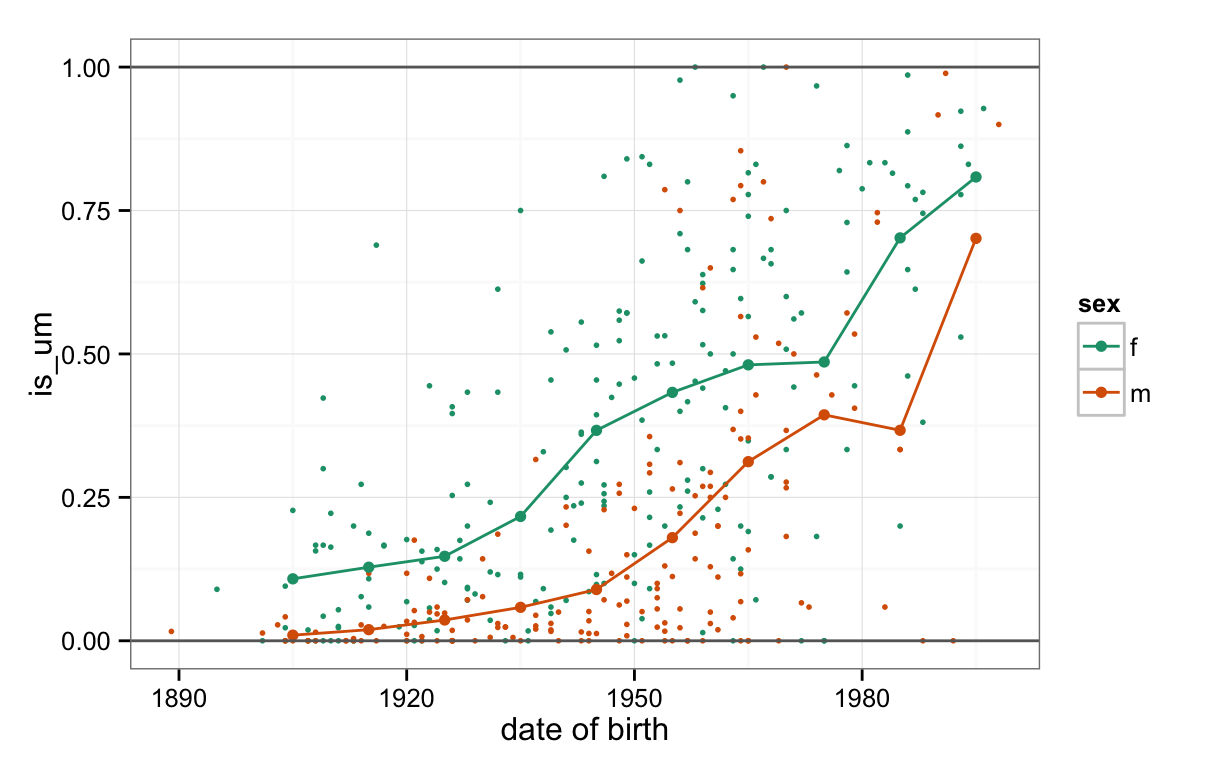
\includegraphics[width=1.16\textwidth]{um.png}
	
	
%\end{frame}



\begin{frame}
\frametitle{Outline}
\tableofcontents
\end{frame}

\section{Specialization and Survival}

\subsection{The Principle of Contrast and dimensions of specialization}

\begin{frame}
\frametitle{Diachronic Blocking Effect}
\begin{block}{``Blocking Effect'' \citep{aronoff1976}}
	\begin{itemize}
		\item General pressure against two forms existing for one function (``doublet''), forcing them to resolve in \textbf{replacement} or \textbf{specialization} \citep{kroch1994}.
		\item[ ]\{\textsl{lough, laughed}\} (laugh-\textsc{pst}; ME, \citealt{taylor1994})\\ \{\textsl{melted, molten}\} (PDE participle, adj pass)\\ \{\textsl{jimmies, sprinkles}\} (candy topping, Philadelphia)
		%\item The possible historical outcomes of a doublet are replacement (one form left) or specialization (forms diverge in function).
	\end{itemize}
\end{block}
\begin{block}{``Principle of Contrast''}
	\begin{itemize}
		\item A strategy that children use in acquiring language: assume that two forms have two meanings (or contexts)\citep[][{ \it inter alia}]{clark1987, clark1990}.
		\item Children hypothesize that novel words also refer to novel objects.
	\end{itemize}
\end{block}
%\begin{itemize}
%	\item General cognitive pressure against two forms existing for one function (``doublet''). 
%	\item This is the ``blocking effect'', as described for morphosyntactic doublets in Kroch (1994).\nocite{kroch1994}
%	\item The possible historical outcomes of a doublet are replacement (one form left) or specialization (forms diverge in function).
%	\item Crucially, they do not coexist forever, nor does one variant die randomly.
%	\item Part of the blocking effect is a language acquisition strategy, the ``Principle of Contrast'' (E. Clark 1987); \citep[cf. also][and references therein]{clark1990}. \nocite{clark1987}
%\end{itemize}
\end{frame}






\begin{frame}
\frametitle{The Principle of Contrast (PrinCon)}
\begin{itemize}
	%\item A strategy that children use in acquiring language: assume that two forms have two meanings (or uses) (first stated in E. Clark 1987).
	\item Demonstrated in experiments such as \citet{markmanwachtel1988, bionetal2013}; see also nuanced review in \citet{bionetal2013}.
		\begin{enumerate}
			\item 20 children
			\item 6 pairs of one familiar item (banana, cow, cup, plate, saw, spoon) and one unfamiliar item (cherry pitter, odd shaped wicker container, lemon wedgepress, radish rosette maker, studfinder, tongs).
			\item \textbf{Control}: ``Show me one''
			\item \textbf{Test}: ``Show me the X'' (X = nonsense syllable)
		\end{enumerate}
	\item Control children pick the unfamiliar object at chance levels, but test children choose unfamiliar objects significantly higher than chance.
\end{itemize}
\end{frame}



\begin{frame}{...and observational results}
		\begin{exe}
			\ex Mo (at the fish-counter): That's a trout.\\
			 D (aged 2:5,1): That's a fish. That not a trout.\\
			 Mo: Well, a trout's a kind of fish.\\
			 D (pause, then pointing at a row of crabs): crabs are a kind of fish.\\
			 \citet[][97]{clark1995}
		\end{exe}
		
		
		
\end{frame}



\begin{frame}
\frametitle{Blocking = Contrast + Evolutionary Dynamics}
\begin{itemize}
	\item A doublet is two variants competing for finite resources (``competing grammars''), as in e.g. biological evolution.
		\begin{itemize} 
			\item Instead of competing for something like food, they are competing for use (time in the mouths/brains of speakers). 
			

			\end{itemize}
	\item Either one variant has a selectional advantage, and so \textbf{replaces} the other. 	
	\begin{itemize} \item \small{cf. \citet[][and subs.]{yang2000, yang2002}, \citet{heycockwallenberg2013}}

			\end{itemize}
	\item Or neither variant has an advantage (or much of one), in which case neutral change, drift (which can also lead to \textbf{replacement}; \citealt{kauhanen2016}).
	

	\item In language learning, the PrinCon means learners can pull apart the contexts of the variants, removing the competition through \textbf{specialization}.
\end{itemize}
\end{frame}


\begin{frame}{Example: Embedded Polar Questions}
		In all stages of English (and in historical Icelandic), a disjunction favors {\it whether} (Bailey, Wallenberg, \& van der Wurff 2012). \nocite{baileywallenbergwurff2012}
	\begin{block}{English}
		\begin{itemize}
		\item[ ]\textbf{Disjunction:}
		\begin{exe}
			\ex I wonder \{{\bf whether},if\} John or Bill is bringing coffee.
			\ex I wonder \{{\bf whether},if\} John is bringing tea or coffee.
			%\ex I wonder \{whether,if\} John is bringing tea or not.
		\end{exe}
		\item[ ]\textbf{Simple:}
		\begin{exe}
			\ex I wonder \{whether, {\bf if}\} Bill is bringing coffee.
		\end{exe}
		\end{itemize}
	
	\end{block}
\end{frame}

\begin{frame}{Slow Specialization of \textsl{whether/if} (N = 1929 clauses)} 


\begin{center}
 \small{Parsed Corpora: YCOE, PPCME2, PPCEME, PPCMBE \nocite{ycoe,ppcme2,ppceme,ppcmbe}}

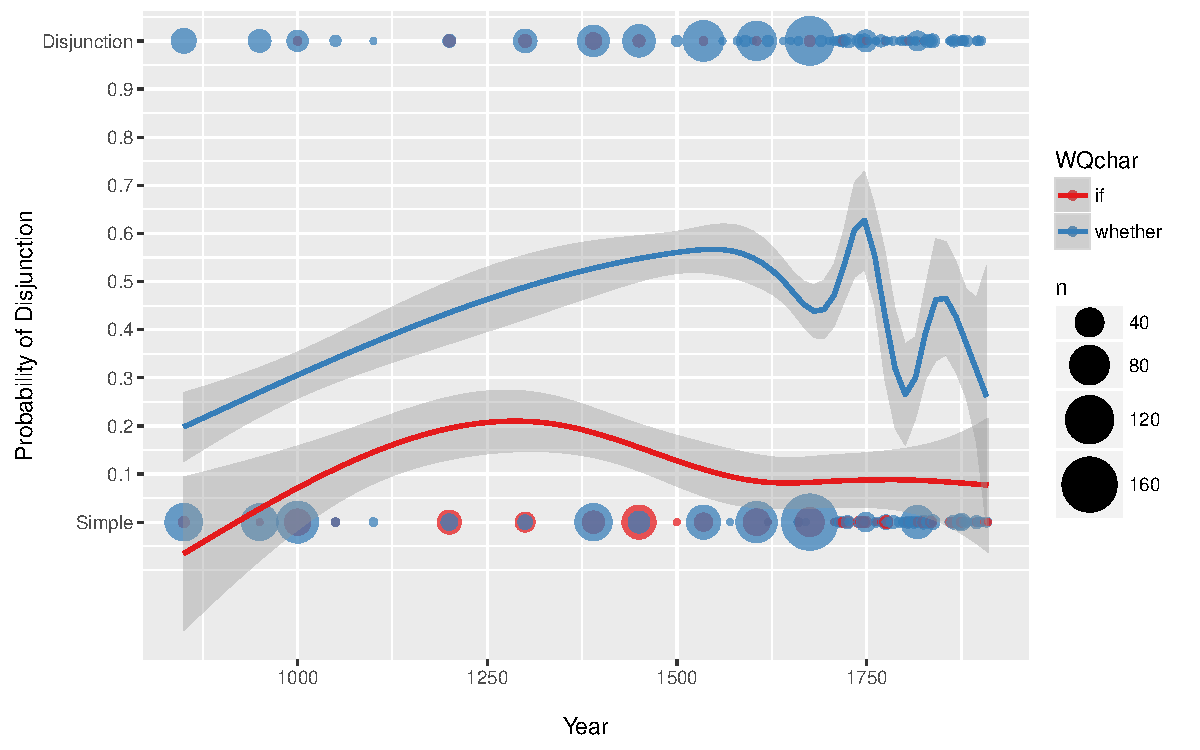
\includegraphics[width=1.1\textwidth]{whetherifEngDisjByYear.pdf}

\end{center}
\end{frame}

\begin{frame}{\textsl{whether/if} replacement slowed/arrested\\\small{(N = 1929 clauses)}}


%\begin{center}
 %\small{Parsed Corpora: YCOE, PPCME2, PPCEME, PPCMBE \nocite{ycoe,ppcme2,ppceme,ppcmbe}}

\includegraphics[width=1.1\textwidth]{whetherifEngWQByYearUnbinned.pdf}

%\end{center}
\end{frame}


%\begin{frame}
%\frametitle{Doublets = Competing Grammars \citep{kroch1994}}
%\begin{itemize}
%	\item[ ] \textbf{``Competing Grammars'', general form}: 2 variants are available to a speaker, in the relevant inventory of grammatical formatives, with \textbf{overlapping} functions (e.g. overlapping meaning).
%		\begin{itemize}
%			\item E.g. two featural versions of the same syntactic head. 
%			\item E.g. two different output mappings for the same phonological input.
%			\item E.g. two different Spell-outs of a morpheme.
%			\item E.g. two different adjunction sites.
%		\end{itemize}
%	\item[ ] A fact about language use: at some point in the derivation, the speaker reaches a \textbf{decision-point}.
%		\begin{itemize}
%		\item The speaker has a choice between formatives to continue the derivation, and either will result in a grammatical utterance, and a meaning close enough to the speaker's intention (the resulting meanings overlap).
%		\item It is speaker ``choice'' more in the sense of an urn problem.
%		\end{itemize}
		%SAY: the decision point exists because the different formatives exist, and that is competing grammars. Note that if they don't overlap in meaning, then the situation still exists formally, but there is no real decision 
		%Say something about adjunction
%\end{itemize}
%\end{frame}



%\begin{frame}
%\frametitle{Doublets = Competing Grammars}
%\begin{itemize}
%	\item Necessary for the description of \textbf{any} linguistic change in a categorical dimension.
%		\begin{itemize} 
%			\item E.g. word-order parameters \citep{pintzuk1991, santorini1992}; a phonological rule like German final stop devoicing (Fruehwald, Gress-Wright, \& Wallenberg 2009)\nocite{fruehwaldgresswallenberg2013}. 
%			\item In any such case, a speaker in the middle of the change in progress (code-)switches between categorical variants \citep{kroch1989}.
%		\end{itemize} 
%\end{itemize}
%\end{frame}


%\begin{frame}
%\frametitle{Summary: Blocking and Contrast}
%So, doublets are Competing Grammars, and Contrast plus evolutionary dynamics yield the outcomes \textbf{replacement} and \textbf{specialization}.\\
%\vspace*{10mm}
%Whether replacement occurs depends on whether specialization can arrest it.

%\end{frame}


\begin{frame}
\frametitle{Consequence: Blocking and Contrast}
\begin{itemize}
	\item A change can be:
		\begin{enumerate}
			\item A replacement change in progress (outright competition going to completion).
			\item A specialization change in progress (specialization for different functions).
			%\item \textbf{``Stable'' variation:} variants have \textbf{imperfectly specialized} along a continuous (or ordinal) dimension, e.g. style, prosodic weight. 
		\end{enumerate}
	\item If categorical variants specialize along a categorical dimension, complete specialization should eventually result.
	\item If categorical variants specialize along a continuous or ordinal dimension, then complete specialization can \textbf{never} result, but replacement can be slowed by \textbf{imperfect specialization}.
\end{itemize}

\end{frame}


\begin{frame}
\frametitle{Specialization along categorical and continuous dimensions}

\begin{center}
\includegraphics[width=1.1\textwidth]{specSchem.png}\\
(figure from Fruehwald \& Wallenberg \textsl{in prep})\nocite{fruehwaldwallenberginprep}
\end{center}

\end{frame}





\subsection{Imperfect Specialization}
%\subsection{The loss of relative clause extraposition}

\begin{frame}{A Very Slow Change}
\begin{itemize}
    \item One consequence of our overall hypothesis is that some things that didn't look like change turn out to be.
    \item Relative clause extraposition is a change in progress, but a very slow one \small{\citep[][]{wallenbergForthcoming, wallenberg2013b, fruehwaldwallenberginprep}}.
        \begin{itemize}
        \item It has been mischaracterized as syntactic optionality.
        \end{itemize}
    \item The study used the same coding query (with minor adaptation) on 7 parsed diachronic corpora (4 language histories).
    \item Both the time-depth and cross-linguistic dimensions were necessary in order to discover the change.
    \item Only because we had both dimensions were we able to observe (and confirm) the slowest syntactic change discovered to date.
    \end{itemize}
\end{frame}

\begin{frame}{Case Study: Relative Clause Extraposition}

%	\begin{block}{French}
%		\begin{exe}
%			\ex \gll mais l'heure vient $[$que je ne parleray plus a vous en proverbes$]$\\
%			but {the time} comes { }that I \sc{neg} speak-\sc{fut} more to you in proverbs\\
%			\quad ``The time approaches when I will no longer speak to you in parables''\\
%			(MCVF, 1523-NEW-TESTAMENT-P, A5V.2491)
%		\end{exe}
%	\end{block}
	
\begin{block}{Icelandic}
		\begin{exe}
			\ex \gll stjarna væri sén í landnorðri frá Jemen, $[$er Kómeta heitir$]$\\
			star was-\sc{subj} seen in northeast from Yemen that Comet is-called\\
			\quad ``A star would have been seen in the northeast from Yemen that's called a Comet\\
			(1861.ORRUSTA.NAR-FIC,.784)\\
		\end{exe}
	\end{block} 

	\begin{block}{English}
		\begin{exe}
			\ex All had now been tried $[$which either threats or promises, forbearance or
fatherly chastisement, could effect$]$.\\
			(PPCMBE, FROUDE-1830,2,2.20; date: 1830)
		\end{exe}
	\end{block}



\end{frame}


%\begin{frame}{Case Study: Relative Clause Extraposition}


%\begin{block}{Icelandic}
%		\begin{exe}
%			\ex \gll stjarna væri sén í landnorðri frá Jemen, er Kómeta heitir\\
%			star was-pst-subj seen in northeast from Yemen, Comp comet calls\\
%			\quad ``A star could have been seen in the northeast from Yemen that is called `comet' ''\\
%			(1861.ORRUSTA.NAR-FIC,.784)
%		\end{exe}
%	\end{block}

%\end{frame}


\begin{frame}{Hypotheses for the diachronic study}
\begin{center}
    \textbf{Hypothesis:} Relative clause position (a binary variable) is specialized along a continuous dimension, weight, and so it should be \textbf{nearly} stable, but not entirely stable.
    \end{center}
%            \begin{itemize}
   %     \item \textbf{Theory:} all variation is really change, competition between variants \small{\citep{kroch1989}}, of some kind.
   %     \end{itemize}
%    \item \textbf{Hypothesis 2:} All IE relative clauses derive historically from clause-adjoined relatives \small{\citep{kiparsky1995}}.
%        \item \textbf{Hypothesis/Suggestion 2':} The old clause-adjoined kind are still around, in the form of extraposition, and the change Kiparsky proposed hasn't finished yet \small{\citep{wallenbergForthcoming}}.
   % \end{itemize}

\end{frame}



%\subsection{Specialization for weight}

%\begin{frame}{Specialization within individuals}
%\begin{itemize}
%	\item Relative clause extraposition in the Parsed Corpus of Early English Correspondence  (PCEEC; \citealt{pceec}).
%	\item Allows us to look at reasonable samples from individual speakers (letter-writers), as well as an historical sample from 1400--1700.
%	\item Coded for prosodic weight of the relative clause, in number of words, from 0--50.
%	\item Also coded for extraposition from Subject vs. Object.
%\end{itemize}
%	\textbf{Hypothesis:} individual speakers treat weight as a continuous variable, with extraposition specialized imperfectly along it \citep[as suggested by][]{antonmackenzie2011a}.

%\end{frame}


%Splice in two plots of speakers


%\begin{frame}{All PCEEC, over time (N = 8073 clauses)}

%\begin{center}
%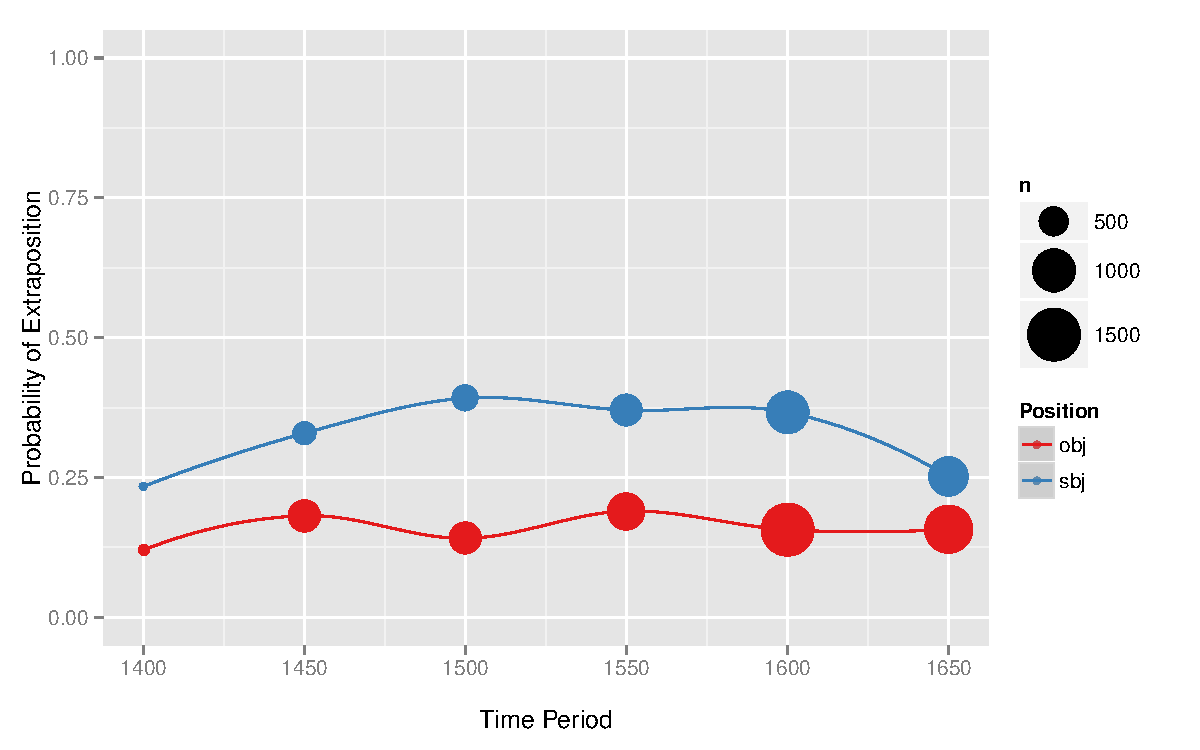
\includegraphics[width=1.1\textwidth]{exSbjObjYearBinned50.pdf}
%\end{center}
%\end{frame}







\begin{frame}{Diachronically, Crosslinguistically}
\begin{itemize}
	\item \textbf{English:} YCOE \citep{ycoe}, PPCME2 \citep{ppcme2}, PPCEME \citep{ppceme}, PPCMBE \citep{ppcmbe}.
	\item \textbf{Icelandic:} IcePaHC \\(Wallenberg, A.K. Ingason, E.F. Sigurðsson, and E. Rögnvaldsson, 2011)\nocite{icepahc09}.
	\item \textbf{Old/Middle French:} MCVF \citep{mcvf}.
	\item \textbf{Historical Portuguese:} Tycho Brahe Corpus of Historical Portuguese \citep{tychobrahe}.
	\end{itemize}
%	\textbf{Hypothesis 1:} the specialization for weight has stabilized, so the effect of weight will be constant over time. \textbf{(Confirmed!)}
%	\textbf{Hypothesis:} the overall rate of relative extraposition will be stable (or without interpretable trend) over time. \textbf{(Rejected!)}

\end{frame}

%\begin{frame}{English, over time (N = 18530 clauses)}

%\begin{center}

%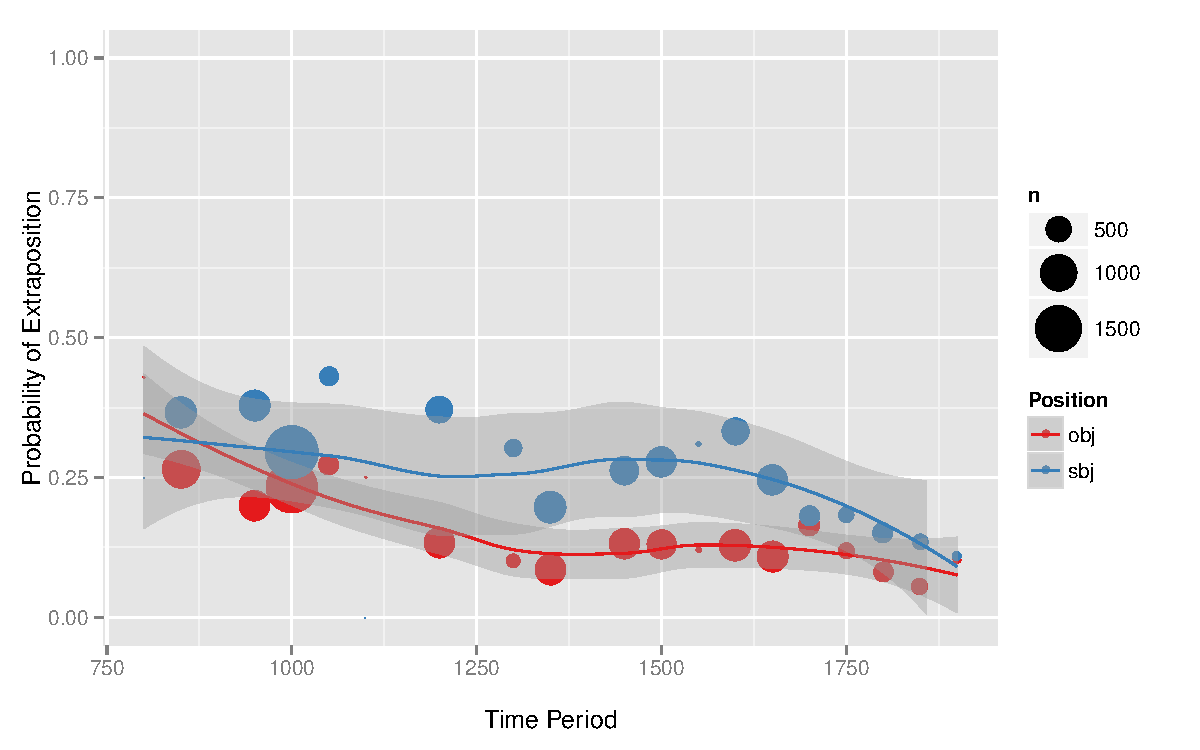
\includegraphics[width=1.1\textwidth]{exSbjObjYearBinned50Loessymeb.pdf}
%\end{center}
%\end{frame}

%\begin{frame}{cf. Yiddish Tense, N = 1030 clauses \\ \small{\citet{wallenberg2013}, building on \citet{santorini1993a}}}

%\begin{center}
%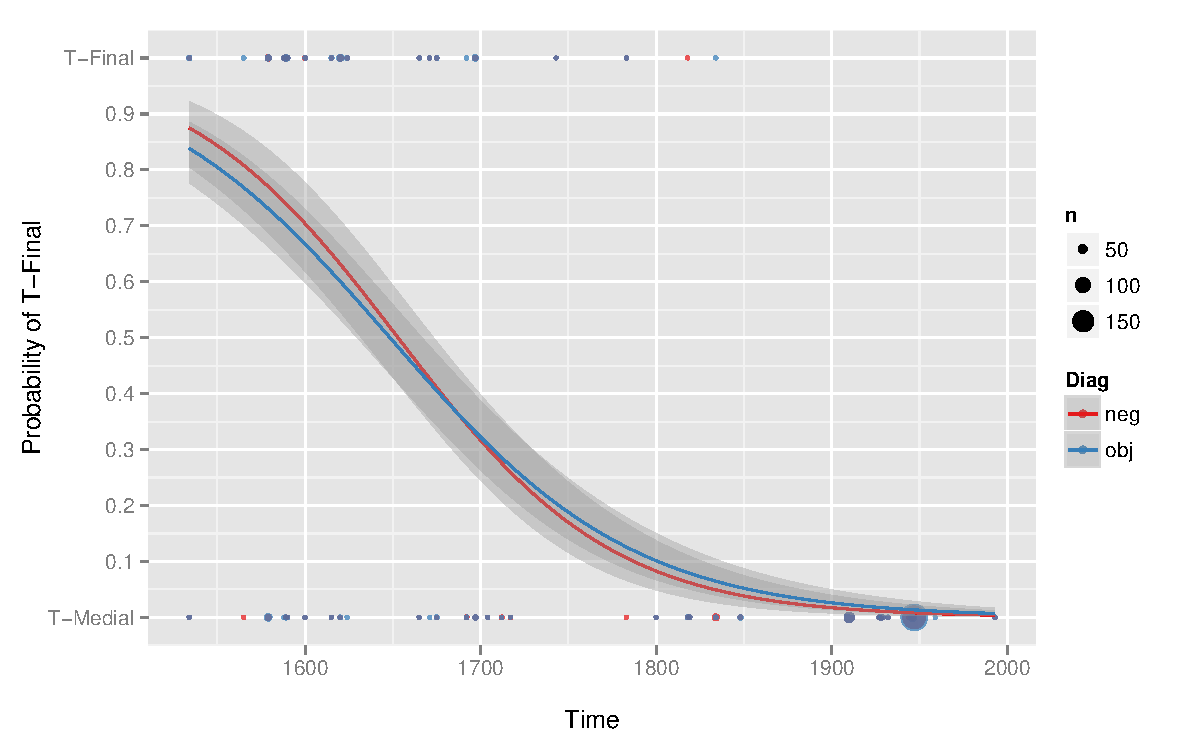
\includegraphics[width=1.05\textwidth]{yiddishLogistic.pdf}
%\end{center}
%\end{frame}





%\begin{frame}{English, average weight over time (N = 18530)}

%\begin{center}
%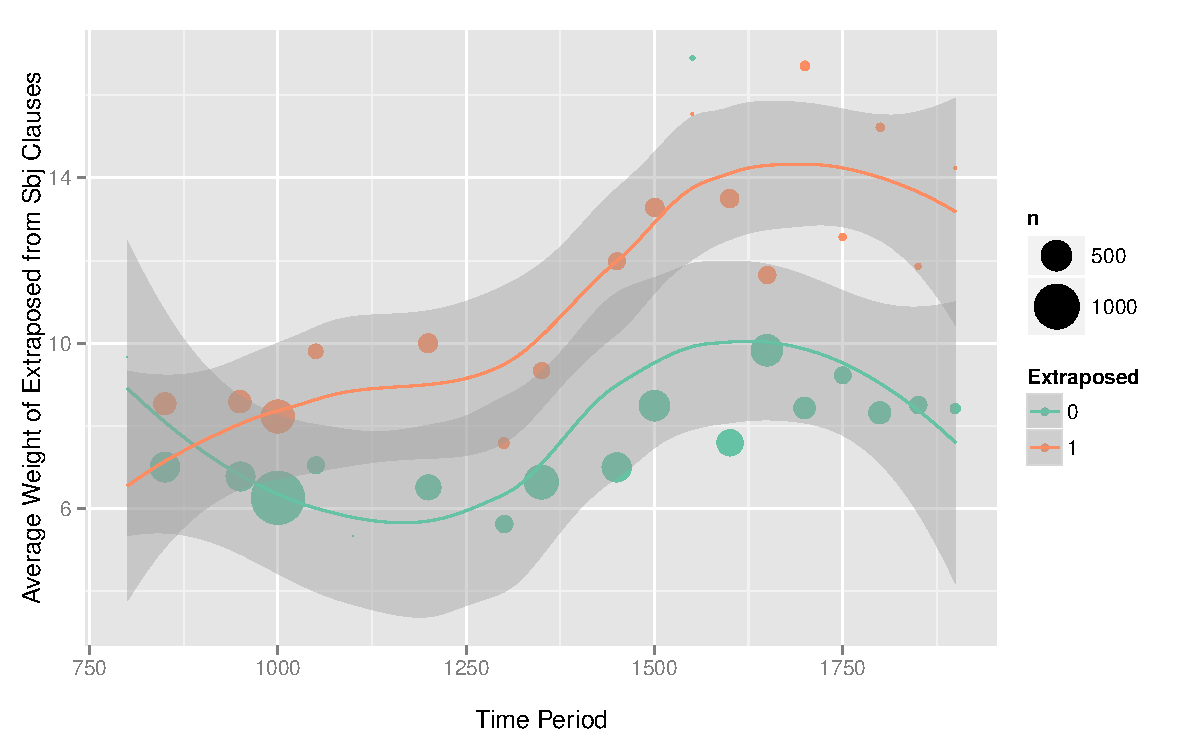
\includegraphics[width=1.1\textwidth]{exWeightYearBinned50Loessymeb.pdf}
%\end{center}
%\end{frame}

%\begin{frame}{Icelandic, over time (N = 3486)}

%\begin{center}
%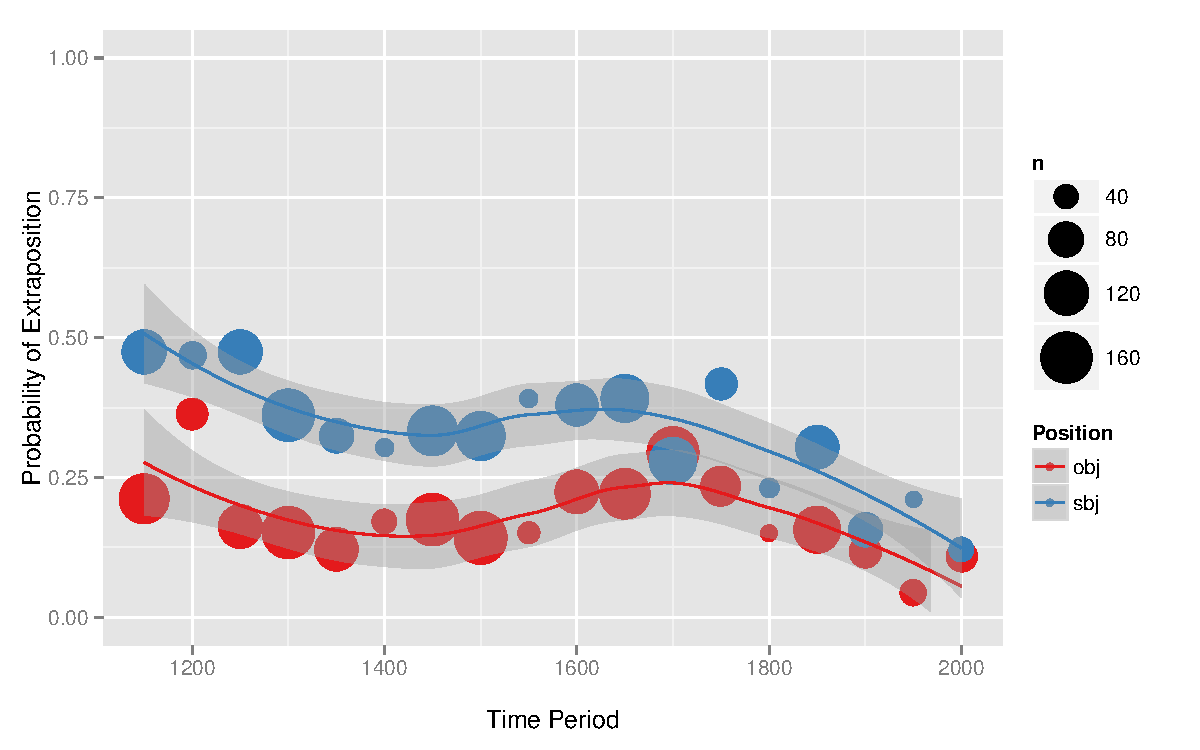
\includegraphics[width=1.1\textwidth]{exSbjObjYearBinned50Loessice.pdf}
%\end{center}
%\end{frame}


%\begin{frame}{Icelandic, average weight over time (N = 3486)}

%\begin{center}
%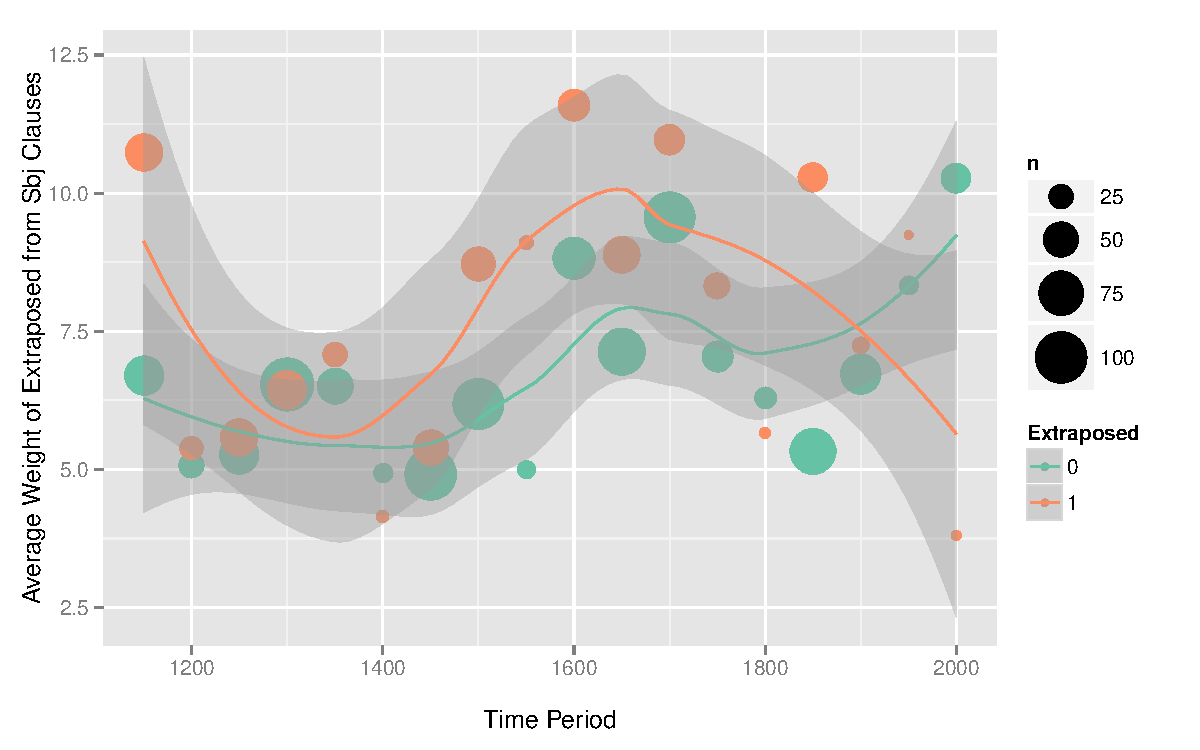
\includegraphics[width=1.1\textwidth]{exWeightYearBinned50Loessice.pdf}
%\end{center}
%\end{frame}



%\begin{frame}{Old/Middle French, over time (N = 8207)}

%\begin{center}
%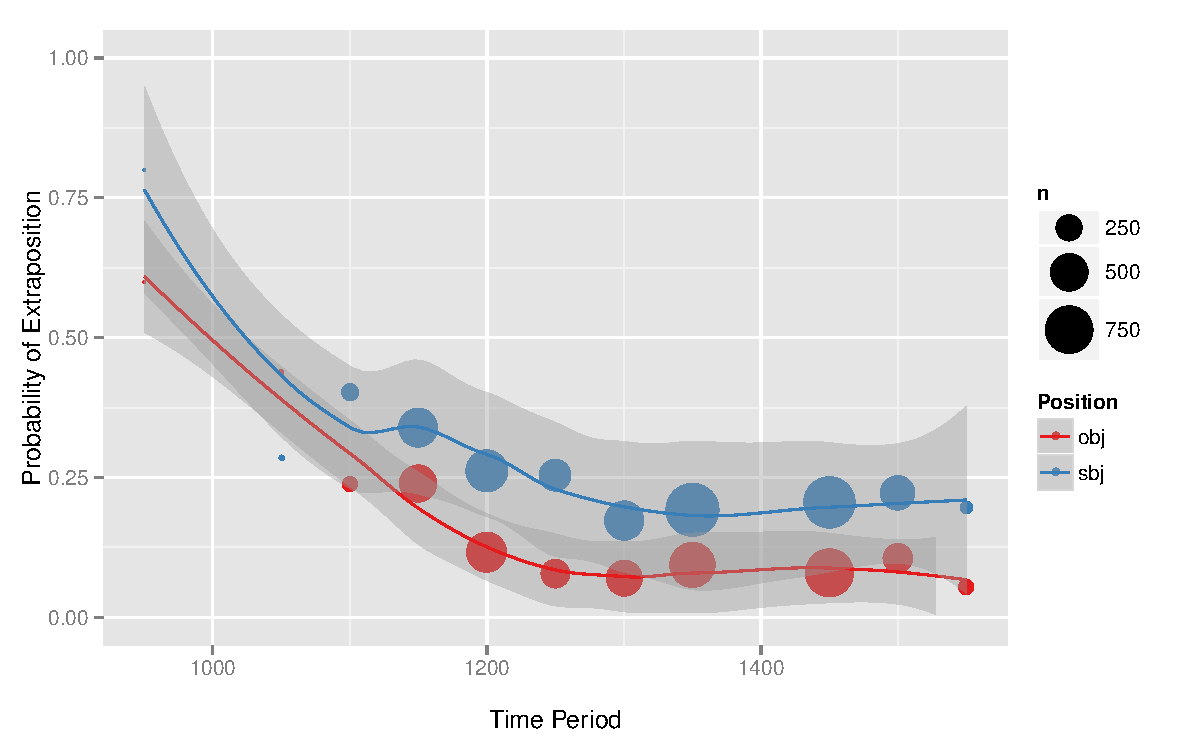
\includegraphics[width=1.1\textwidth]{exSbjObjYearBinned50Loessfre.pdf}
%\end{center}
%\end{frame}


%\begin{frame}{French, average weight over time (N = 8207)}

%\begin{center}
%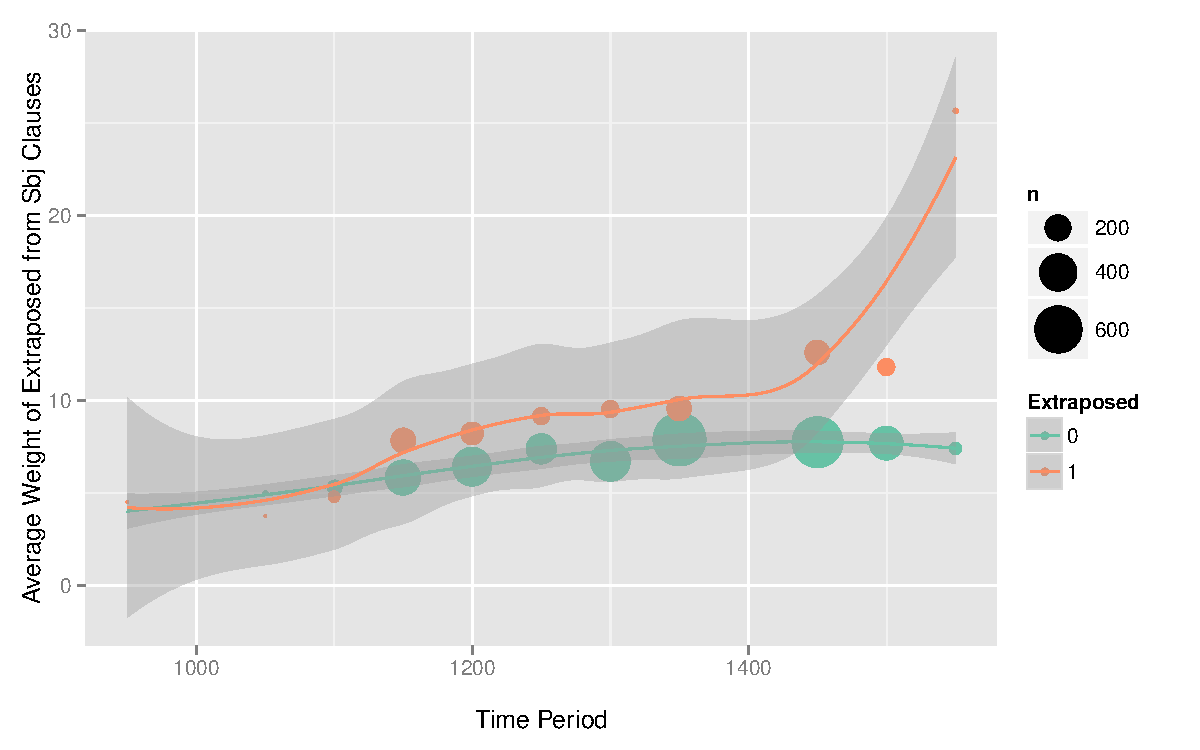
\includegraphics[width=1.1\textwidth]{exWeightYearBinned50Loessfre.pdf}
%\end{center}
%\end{frame}

%\begin{frame}{Portuguese, over time (N = 2398)}

%\begin{center}
%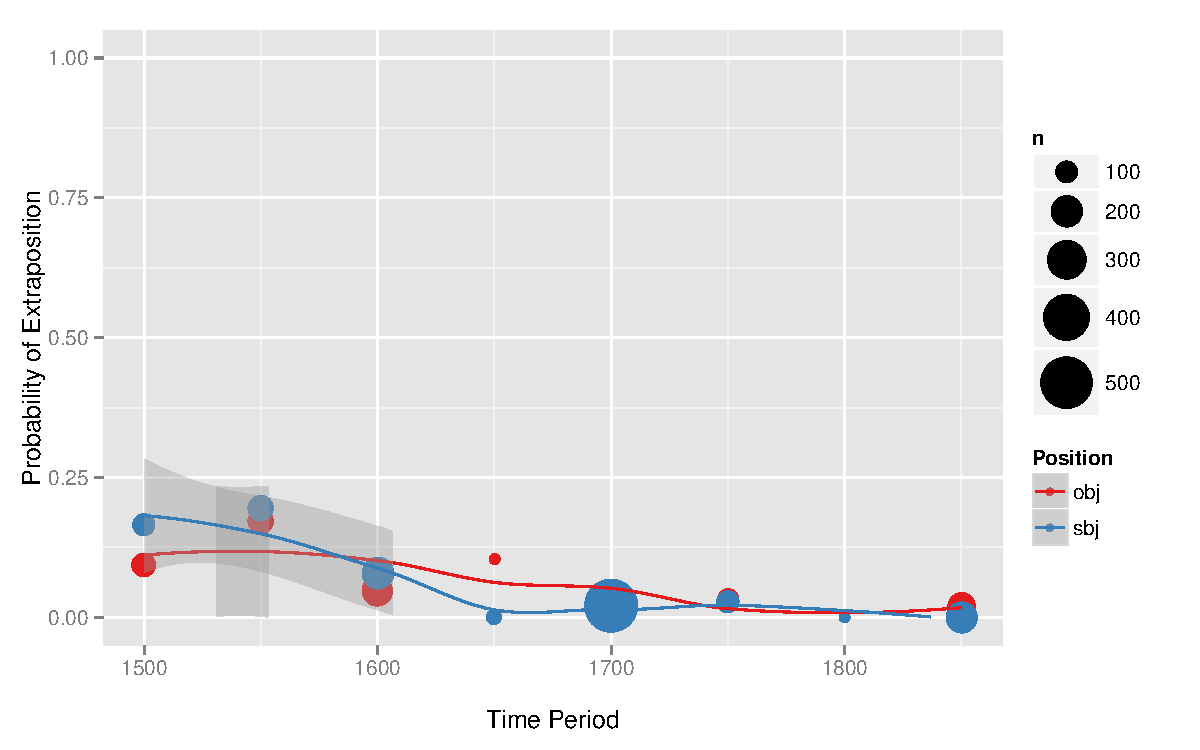
\includegraphics[width=1.1\textwidth]{exSbjObjYearBinned50Loessport.pdf}
%\end{center}
%\end{frame}


%\begin{frame}{Portuguese, average weight over time (N = 2398)}

%\begin{center}
%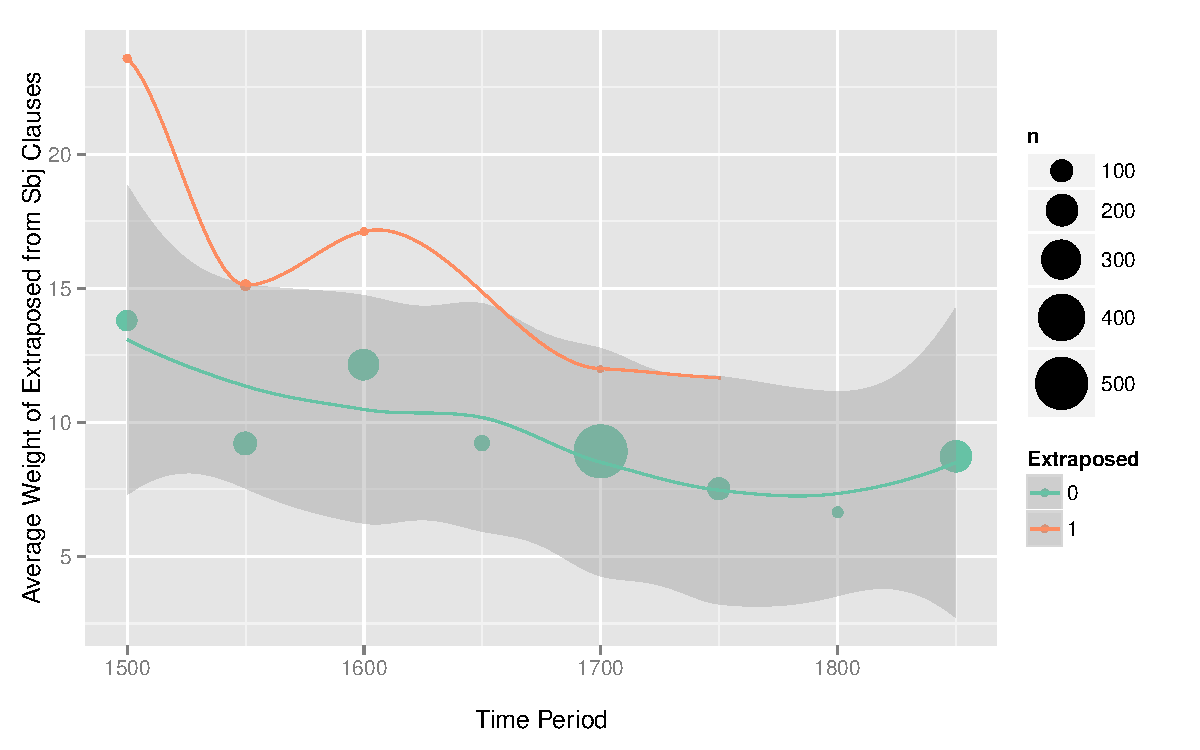
\includegraphics[width=1.1\textwidth]{exWeightYearBinned50Loessport.pdf}
%\end{center}
%\end{frame}





\begin{frame}{Four Languages (Subj Ex), over time}

\begin{center}
\includegraphics[width=1.1\textwidth]{exYearBinned50Loessall.pdf}
\end{center}
\end{frame}

\begin{frame}{Statistical characteristics of the change}
    \begin{itemize}
    	\item The slope of the decline over time is shallow; slopes for Icelandic, English, French, and Portuguese = -0.37, -0.36, -0.32, -1.24 from Subject\\(based on mixed effects logistic regression controlling for weight and other factors).
	\item Weight has a significant effect in each language, but the effect doesn't change over time.
%	\item Icelandic, English, and French show very similar same rate of change for EX (a kind of Constant Rate Effect?)  \\\small{(model comparison not possible for computational reasons with the mixed effects models; p = 0.47 for Icelandic and English with standard regression)}.
\end{itemize}
\end{frame}

%\begin{frame}{The origin of the slow change?}
%    \begin{exe}

%\ex \label{vediccar1} \gll \textbf{yó} \textbf{mártya\d{h}} \textbf{śíś\={i}te} \textbf{áty} \textbf{aktúbhir}, \textbf{m\={\'{a}}} na\d{h} sá ripúr \={i}śata \\
%which mortal sharpen-Mid-Sg overly nights-\sc{instr}, not us-\sc{gen} that trickster dominate-Subj3Sg\\
%\quad ``As for the mortal who makes himself too sharp by night, may that trickster not gain power over us''\\
%\citep[RV 1.36.16, cited in][156]{kiparsky1995}
%\end{exe}
%\end{frame}


%\begin{frame}{The origin of the slow change?}
%\begin{exe}
%         \ex \label{engcar1} By God's blessing I calculate that the Spirit of Dishonesty shall not get dominion over me; nor the Spirit of %Despondency, nor any other evil spirit; \textbf{in which case
%all will and must be well}.\\
%(Letter by Thomas Carlyle, date: 1835; ID CARLYLE-1835,2,266.176 in PPCMBE)
%        \ex \label{engcar3} Nowadays, however, flowers can be arranged in various styles -- some flat, some slightly raised, some bunched %boldly in certain
%places and forming the piece de resistance of
%the whole work -- \textbf{all of which variations depend upon the artistic
%perceptions of the operator\textbf}.\\
%        (\textsl{Commercial gardening...}, date: 1913;ID WEATHERS-1913,1,9.217 in PPCMBE)
%\end{exe}
%\end{frame}


\begin{frame}{Summary: Change in Extraposition}

\begin{itemize}
\item \textbf{Why the change?} After actuation, extraposition and \textsl{in situ} are competing variants in use, so there can't not be a change, even with partial specialization.
		\begin{itemize}
		\item Specialization can only be partial along the (continuous) weight dimension.
		%\item Perhaps a small selectional advantage has asserted itself in the usage-overlap, but can only do so slowly because the overlap is limited.
		\end{itemize}
	\item The change is slow enough to be not observable without considerable time-depth.
%	\item Perhaps \citet{kiparsky1995} identifies a change that goes back to Proto-Germanic, though hard to test.
%	\item The questions we can ask are now far more nuanced, given cross-linguistic and extended diachronic dimensions.
\end{itemize}

\end{frame}





\section{Morpho-lexical Case Study}
\subsection{How fast does specialization take place?}

\begin{frame}{Charles's Question (or Yang's Paradox?)}
		\begin{center}
			Experimental results on word-learning show the Principle of Contrast differentiates words nearly instantaneously. The PrinCon is too fast to produce the slow specialization we see in, e.g. syntax. Is there another pressure?\\
			\vspace*{2mm}
			\small{(Caveat: \citet{bionetal2013} show retention of the new mapping is not instantaneous, and not reliable until after 24 months of age.)}\\
			\vspace*{5mm}
			\large{So, is it really true that word/morpheme specialization happens very quickly? And if not, what about the experimental evidence?}
		\end{center}
\end{frame}



\begin{frame}{\textsl{melted/molten} specialization}
\begin{itemize}
\item Variation in participle forms \textsl{gemolten, gemælted} goes back to Old English, with first adnominal use of \textsl{molten} from 1300 (OED).
\item \textsl{molten} in PDE now seems to be fully specialized (and maybe \textsl{melted} as well):
\end{itemize}
\begin{exe}
	\ex The gold was \{melted / *molten\} by the fire. \textbf{((passive) participle context)}
	\ex The fire has  \{melted / *molten\} the gold.\\\textbf{((past) participle context)}
	\ex The \{?melted / molten\} gold flowed down the hill. \textbf{(adjectival or adjectival passive DP-internal context)}
\end{exe}

\end{frame}

\begin{frame}{\textsl{melted/molten} specialization}
\begin{exe}
	\ex The gold was \{melted / *molten\} by the fire. \textbf{(participle context)}
	\ex The \{?melted / molten\} gold flowed down the hill. \textbf{(adjectival context)}
\end{exe}
\begin{itemize}
\item Question: how quickly did this morphological/lexical doublet specialize, in real time?

\item Question: how long did intraspeaker variation persist, in both contexts?
\item Using the {P}enn-{Y}ork {C}omputer-annotated {C}orpus of a {L}arge amount of {E}nglish based on the {TCP (PYCCLE-TCP; \citealt{pyccle})}, roughly 1 billion words.
\end{itemize}
\end{frame}


\begin{frame}{\textsl{melted/molten} specialization N =  7946 tokens}

%\begin{center}
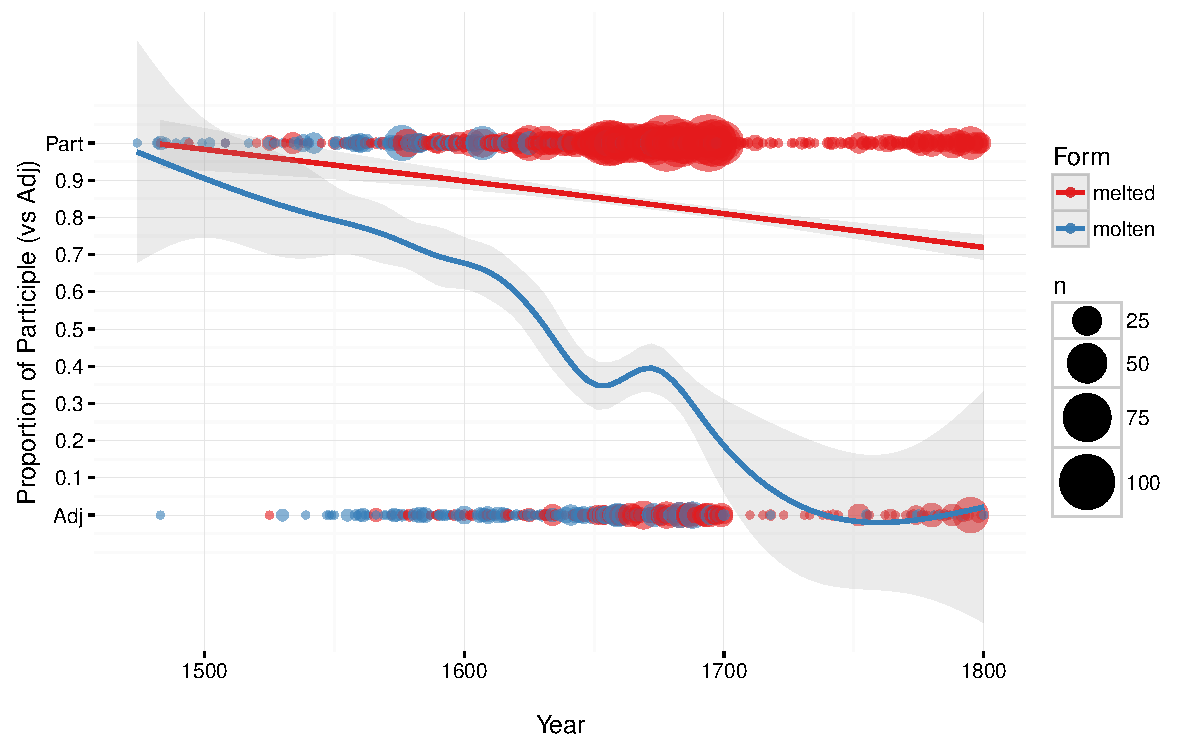
\includegraphics[width=1.128\textwidth]{ContextByDateUnbinnedWithDots2.pdf}
%\end{center}
\end{frame}


\begin{frame}{Simultaneous Replacement? N =  7946 tokens}

%\begin{center}
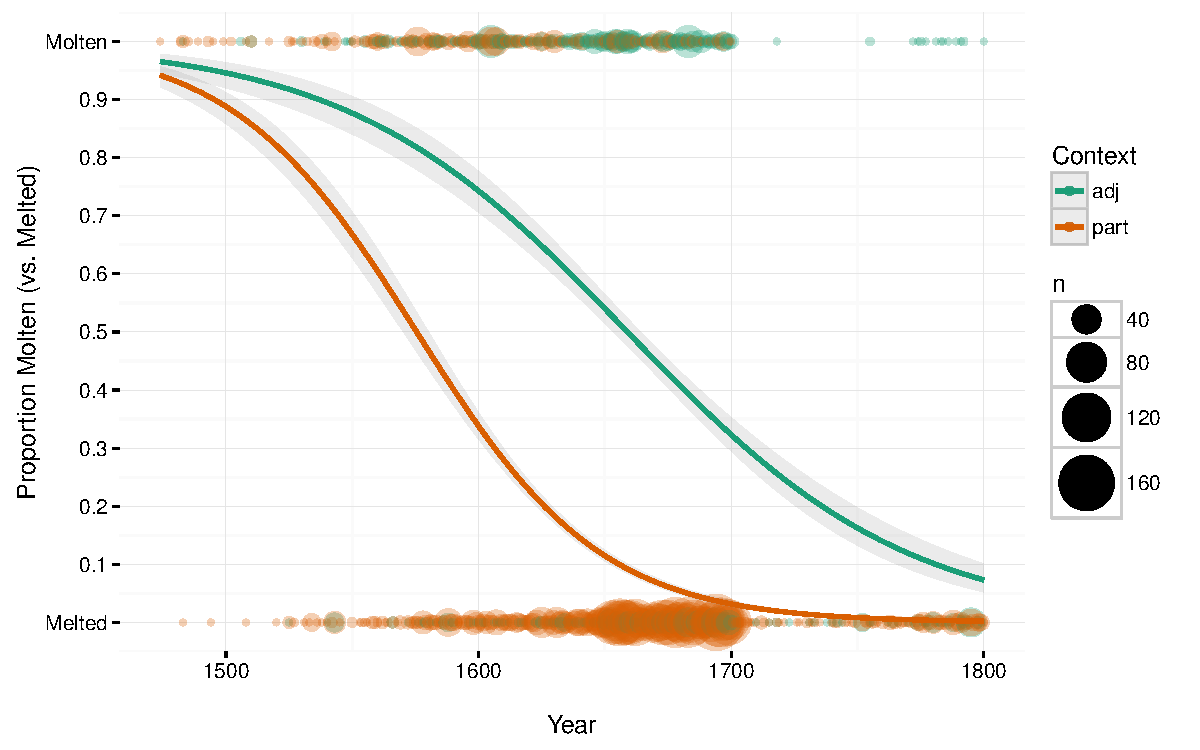
\includegraphics[width=1.128\textwidth]{FormByDateUnbinnedWithDots2.pdf}
%\end{center}
\end{frame}




\begin{frame}{471 identifiable speakers, N = 3601 tokens}

%\begin{center}
%\small{(Note: the differing lengths of green lines, and 1575, 1580, 1601.)}
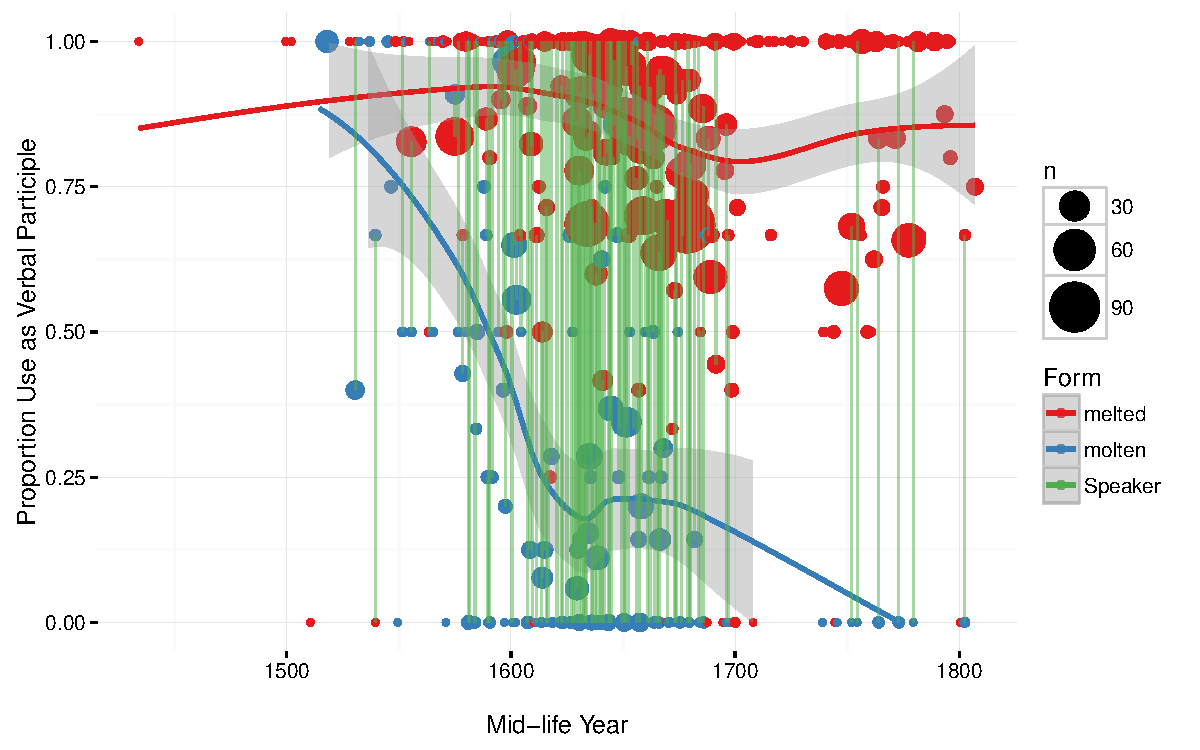
\includegraphics[width=1.128\textwidth]{ContextByDateAuthor.pdf}
%\end{center}%1575, 1601 for good variation, AND POINT OUT LENGTH OF GREEN LINE!
\end{frame}


\begin{frame}{Individual Speakers, 1570-1670 midlifes}

\begin{center}
\small{(Note: the differing lengths of green lines, and 1575, 1580, 1601)}

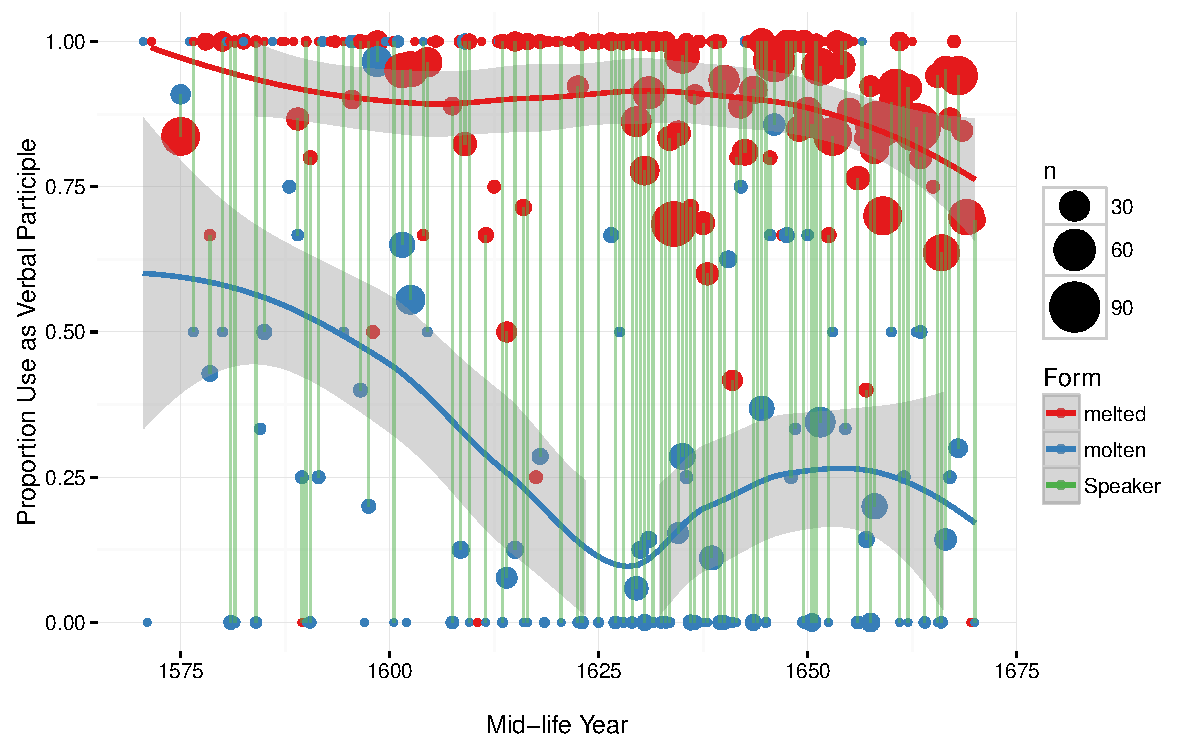
\includegraphics[width=1.128\textwidth]{ContextByDateAuthor1570.pdf}
\end{center}
%1575, 1601 for good variation, AND POINT OUT LENGTH OF GREEN LINE!
\end{frame}

\begin{frame}{Intraspeaker Variation}
		\begin{exe}
			\ex \begin{xlist} \ex Method of breeding Horses...Molten grease and fatning balls\\
			\ex ...which may bring away any melted grease\\
			\end{xlist}
			\ex \begin{xlist} \ex ...the grease is molten into them\\
			\ex ...considering that if grease should be melted\\
			\end{xlist}
			\ex \begin{xlist} \ex...adding thereto some Honey; which being molten , give it the Horse\\
			\ex ...English Honey; and when these are melted, and well stirred together\\
			\end{xlist}
		\end{exe}
		(Robert Almond, \textsl{The English horsman and complete farrier...}, date: 1673)
\end{frame}


\begin{frame}{Solving Yang's Paradox}
		\begin{itemize}
			\item Perhaps the first generation to hear the innovation, Generation 1, does try to specialize completely, if possible.
			\item Generation 1 speakers will not necessarily converge on the same dimension of specialization (and indeed, may mix categorical and continuous dimensions as well).
			\item Generation 2 cannot help but hear true synonyms, given the overlap of use in the community.
			\item Subsequent generations may converge on one dimension of specialization (or a few, again potentially mixing categorical and continuous), but there will be intra- and inter-speaker variation all the way.
		\end{itemize}
\end{frame}


\section{Variational Specialization}
\subsection{Extending Yang (2000, 2002)'s model to specialization}
\begin{frame}{Specialization and Yang's Variational Learning}
		\begin{enumerate}
			\item Identify a domain of specialization:
				\begin{itemize}
					\item \textbf{Actively}, by the child innovating \textsl{de novo}?
					\item \textbf{Passively}, though random sampling of finite populations of utterances?
				\end{itemize}
			\item Allow the variants different (quantitative) representations for different contexts, along the domain of specialization:
			\begin{itemize}
				\item[\textcolor{blue}{a.}] For categorical variants along categorical dimensions, decouple tracked frequencies of variants for each context, C_1,...,C_n, in the dimension of specialization.
				\item[\textcolor{blue}{b.}] For categorical variants along continuous dimensions, decouple tracked mean values (or targets) of variants for the dimension of specialization.
			\end{itemize}
			\item Specialization goes to completion as the learner has variants behave differently in different contexts.		\end{enumerate}
\end{frame}

\begin{frame}{3a. Specialization completes in the categorical-categorical case}
		\begin{itemize}
			\item Suppose Variant A is losing to Variant B due to global selective pressure, but they begin to specialize for C_1 and C_2.
			\item Specialization completes in a categorical dimension:
			\begin{itemize}
				\item \textbf{Actively}, by augmenting the represented frequency of Variant A in C_1 and augmenting Variant B in C_2?
				\item \textbf{Passively}, by allowing whatever evolutionary dynamics hold in the different contexts play out, whether the outcome is different or not?
			\end{itemize}
		\end{itemize}
\end{frame}

\begin{frame}{3b. Specialization completes in the categorical-continuous case}
		\begin{enumerate}
			\item Suppose Variant A is losing to Variant B due to global selective pressure, but they begin to specialize along a continuous dimension C.
			\item Learner allows their mean/target values for C to become distinct: $\mu$_{C_A},  $\mu$_{C_B}
			\item Specialization completes in a continuous dimension:
			\begin{itemize}
				\item \textbf{Actively}, by moving $\mu$_{C_A},  $\mu$_{C_B} away from each other?
				\item \textbf{Passively}, by allowing $\mu$_{C_A},  $\mu$_{C_B} the possibility of moving away from each other?
			\end{itemize}
		\end{enumerate}
\end{frame}


\begin{frame}{Specialization in Acquisition: active or passive?}
		\begin{itemize}
			\item Is there any way to distinguish the two, given that different linguistic cases may have different selectional pressures?
				\begin{itemize}
					\item You can model a lot of scenarios assuming various selectional pressures interacting with various child-driven ``accelerations'' of specialization.
				\end{itemize}
			\item \textbf{Possible hypothesis:} maybe the child-driven amount of manipulating A and B's frequencies is the same per token in every linguistic case, and can be estimated.
			\item Maybe we can identify some true neutral changes, to abstract away from selective pressures \citep{kauhanen2016}.
		\end{itemize}
\end{frame}

%\begin{frame}{Specialization in Acquisition: active or passive?}
		
%		\textbf{Passive Hypothesis:} PrinCon \textbf{is} the decoupling of contexts C_1,...,C_n by learners, and the rest is due to the selective pressures being different in the different contexts, \textbf{once the tracked frequencies are decoupled in the learner's representation of the variation.}
%		\begin{itemize}
%			\item Distinguished from the Constant Rate Effect by the decoupling of tracked frequencies for, e.g. Variant A in C_1,...,C_n.
%			\item Contextual effects within the CRE can be thought of as transformations on a single tracked frequency for Variant A across all contexts.
%		\end{itemize}
%\end{frame}







\section{Conclusion}

%\begin{frame}{Conclusions}
%		\begin{itemize}
%			\item \textbf{Specialization} can allow competing forms to survive, but only if their functions diverge.
%			\item \textbf{Imperfect specialization:} mismatch between categorical variation and continuous dimensions of specialization (or vice-versa) leads to long-term stochastic variation, though not quite stability.
%			\item An extension of \citet{yang2000,yang2002}'s \textbf{variational learning model} provides some specific mathematical hypotheses about specialization in acquisition, which we should test.
%			\item \textbf{PrinCon} has a natural definition in this model, and can be reconciled with the speed of specialization.
%			\item Two things I didn't discuss because of time:
			%\item The information on \textbf{transition} is based on very high-quality, expensive data (parsed diachronic corpora, beyond the ability of an individual to produce).%which allows us to observe a lot more than we could before.
			%\item It is still noisy, and we would like finer resolution as we tackle questions above, and e.g. selection vs. drift.
%		\end{itemize}
%\end{frame}

\begin{frame}{How does it relate to the project?}
		\begin{itemize}
			\item When varieties come into contact, new linguistic forms come into competition with older forms.
			\item Replacement and specialization both play out at an individual and speech community level, simultaneously.
			\begin{itemize}
				\item We need a (mathematical) theory of this.
				\item We need to test quantitative hypotheses.
			\end{itemize}
		\end{itemize}
\end{frame}

\section{Gender} 

\begin{frame}{Now for something completely different: gender}
		\begin{itemize}
		\item \textbf{Linguistic sex/gender effects:} it is well known that speaker-sex has a stochastic effect on the frequency with which linguistic variants are used.
		\item \textbf{Hormonal Organising Effects:} the action of sex steroids during sensitive period for sexual differentiation 
		(\textsl{in utero}, esp. weeks 8-24 for humans), affecting primary/secondary sex characteristics, and:
			\begin{itemize}
				\item \textbf{Brain morphology:} e.g. the sexually-dimorphic nucleus of the pre-optic area in mammals, including humans, with a correlate in birds \citep[see review in][]{balthazart2011}.
				\item \textbf{Behaviour:} mating behaviours in various mammals, pair-bonding and birdsong in birds, \textbf{gender identity} in humans \small{\citep{hinesetal2002, berenbaumbailey2003, hinesetal2004, cohenbendahanetal2005, auyeungetal2009}}, and \textbf{gendered social learning in humans} \citep{hinesetal2016}.
			\end{itemize}
	\end{itemize}
\end{frame}

\begin{frame}{Rise of Pre-aspiration in Tyneside English \\ in 16 women \small{(Cochrane 2016)}}


\begin{center}

\includegraphics[width=1.1\textwidth]{claire.png}

\end{center}
\end{frame}


\begin{frame}{How does it relate to the project?}
		\begin{itemize}
			\item If there are subtle biases in social learning, based on early life hormone exposure (and correlating with continuous gender identity), this will affect the spread of new variants through a population.
			\item If we catch new variants in their early spread, we may see these biases more clearly.
			\item Given the rich sociological information available in Iceland, and the contact situation, we might have a greater opportunity to identify such biases.
		\end{itemize}
\end{frame}


%\begin{frame}{Further questions}
%		\begin{itemize}
%			\item This model of specialization is an extension of \citet{yang2000, yang2002}.
%			\item Can we observe specialization, and the choosing of domains of specialization diachronically?
%			\item Can we observe it in acquisition?
%				\begin{itemize}
%					\item Production data may not be good enough here.
%				\end{itemize}
%			\item Can we observe either well enough to test active vs. passive hypotheses?
%		\end{itemize}
%\end{frame}


\begin{frame}{Acknowledgements}
\begin{center}
Thank you first to Josef Fruehwald for working out many of these ideas with me, and to Anthony Kroch, Betsy Sneller, Charles Yang. Special thanks to Aaron Ecay for help with PYCCLE and Weihnachtsgurke, among other things. Thanks to Jacques Balthazart, Claire Cochrane, Anton Karl Ingason, Laurel Mackenzie, anonymous reviewers, and my RAs and participants.
\vspace{5mm}\\
\url{https://github.com/joelcw/tyneside/tree/master/extraposition}\\\url{https://github.com/joelcw/molten}\\\vspace{3mm}

\includegraphics[scale = 0.1]{ncllogo.jpg} \includegraphics[scale = 0.4]{cbelogo.jpg} 
\end{center}
\end{frame}


\begin{frame}[allowframebreaks]
\frametitle{References}
\newcommand*{\newblock}{natbib}
\bibliographystyle{linquiry2}
\bibliography{joelrefs}
\end{frame}


\begin{frame}{Simultaneous replacement or extreme specialization?}
		\begin{exe}
			\ex \textbf{(\textsl{molten} implies heat in PDE:)}\\
			Is silly putty molten rubber?\\
			\ex \textbf{(\textsl{molten} implies liquidy/sludgy state in PDE:)}\\
			melted spatula vs. molten spatula\\
			\ex \textbf{(both:)}\\
			melted cheese vs. molten cheese\\
			(J. Fruehwald, p.c., for examples above)
			\ex \textbf{(\textsl{molten} implies recognizable substance in PDE:)}\\
			...that the increase and augmentation of Nilus commes of the snowe waters molten and thawed in those regions.\\
			(attr Barnabe Riche, \textsl{The famous hystory of Herodotus...}, date: 1584)
		\end{exe}
		
\end{frame}

\begin{frame}{Model Comparison: specialization by context}

\begin{center}
Model 1: Form \textasciitilde  (1 | file) + (1 | author) + zDate + Context\\
\vspace*{1mm}
Model 2: Form \textasciitilde  (1 | file) + (1 | author) + zDate{  }*{  }Context\\
\vspace*{4mm}

	\begin{tabular}{rrrr}
\toprule
	model & AIC & BIC & p-value (Chisq)\\
	\cmidrule{2-4}
Constant Rate & 3039.1 & 3071.6 & -- \\
with Date*Context &  3032.3 & 3071.3 & 0.003\\
\bottomrule
\end{tabular}
\end{center}
\end{frame}



\begin{frame}{Prediction for an Active Hypothesis}
		\begin{itemize}
			\item[] \textbf{In true neutral change ONLY:} once specialization begins to take place, it should be relentless, and \textbf{symmetrical}, and both variants should always survive (in the cat-cat case).
				\begin{itemize}
					\item The frequency of Variant A in C_1 is always being augmented in lockstep with the punishment of Variant A in C_2. Both will have to survive, and:
					\begin{itemize}
					\item[\textbf{Corollary 1:}] the frequency of Variant A in C_1 and Variant A in C_2 will need to move away from each other.
					\item[\textbf{Corollary 2:}] the probability of C_1 being expressed by Variant A will rise as the probability of C_1 being expressed by Variant B declines.
					\end{itemize}
				\end{itemize}
		\end{itemize}
\end{frame}

\begin{frame}{\textsl{melted/molten}: consider Corollary 1}

%\begin{center}
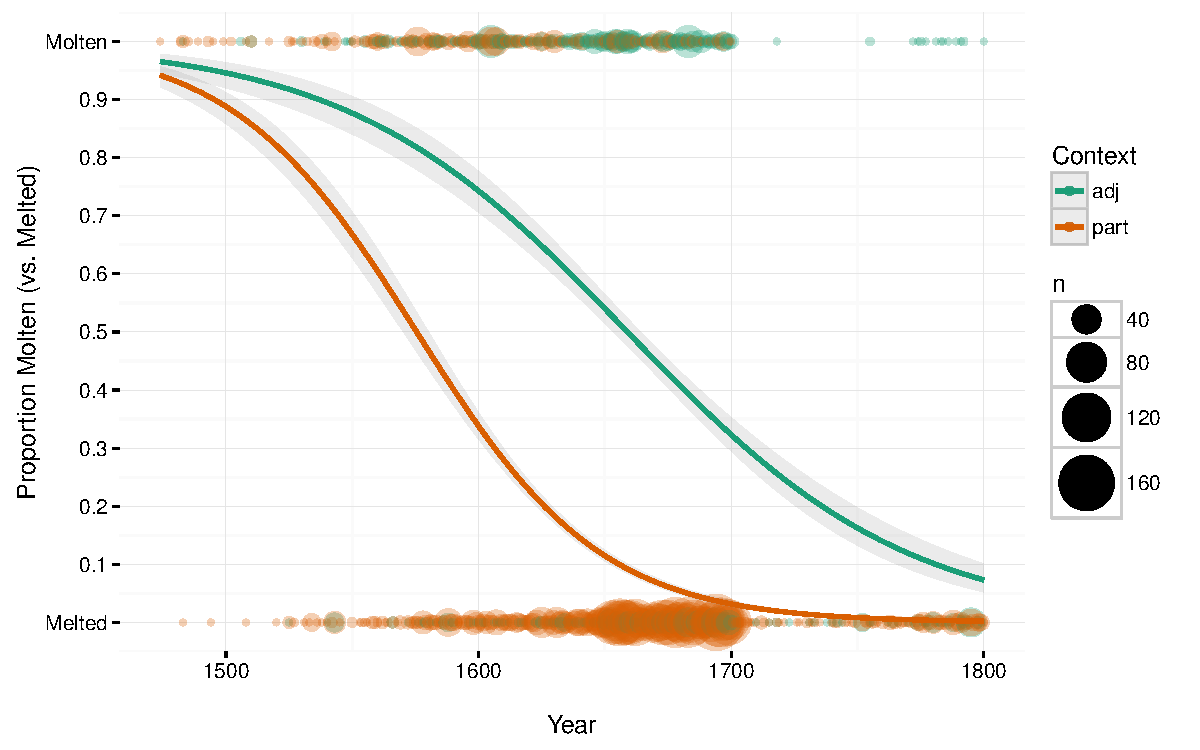
\includegraphics[width=1.128\textwidth]{FormByDateUnbinnedWithDots2.pdf}
%\end{center}
\end{frame}

%\begin{frame}{\textsl{melted/molten}: consider Corollary 2}

%\begin{center}
%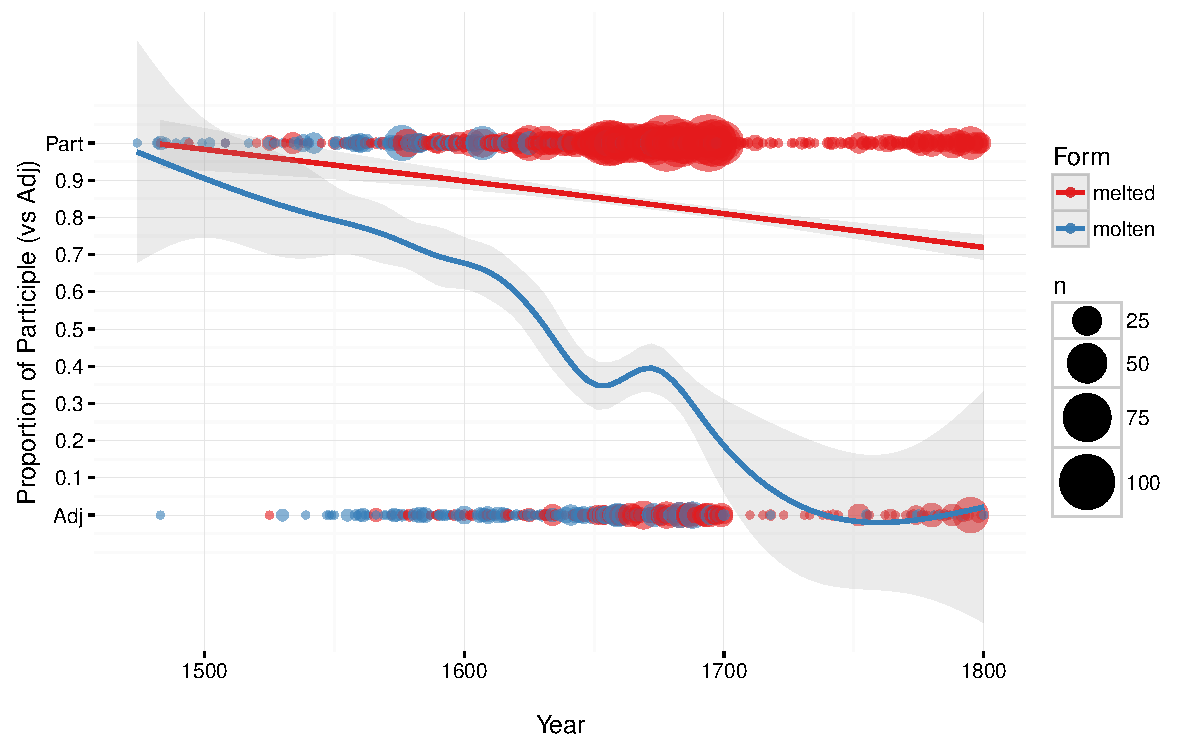
\includegraphics[width=1.128\textwidth]{ContextByDateUnbinnedWithDots2.pdf}
%\end{center}
%\end{frame}


\begin{frame}{But what if there's a global selective pressure for B?}
		\begin{itemize}
			\item Once specialization begins to take place, it is relentless, but not necessarily symmetrical: if Variant A is losing globally, and C_1 and C_2 are decoupled, the amount of augmentation of Variant A in C_1 can be =, >, or < the global selective pressure against Variant A:			
			\begin{itemize}
					\item \textbf{amount of augmentation = selective pressure $\rightarrow$} variation is stable in C_1 and B wins in C_2.\\(THIS SCENARIO IS FULLY BIZARRE: we've now used the PrinCon to engineer stable variation.)
					\item \textbf{augmentation < selective pressure $\rightarrow$} Variant A loses in both C_1 and C_2 but at different rates.
					\item \textbf{augmentation > 2 x selective pressure $\rightarrow$} A wins in C_1 at the same rate B wins in C_2.
					\item \textbf{selective pressure < augmentation < 2 x selective pressure $\rightarrow$} A wins in C_1, but more slowly than B wins in C_2.			
			\end{itemize}
		\end{itemize}
\end{frame}


\begin{frame}{2D:4D ratio: smaller $\rightarrow$ more pre-natal T (or T/E)}
\begin{center}
	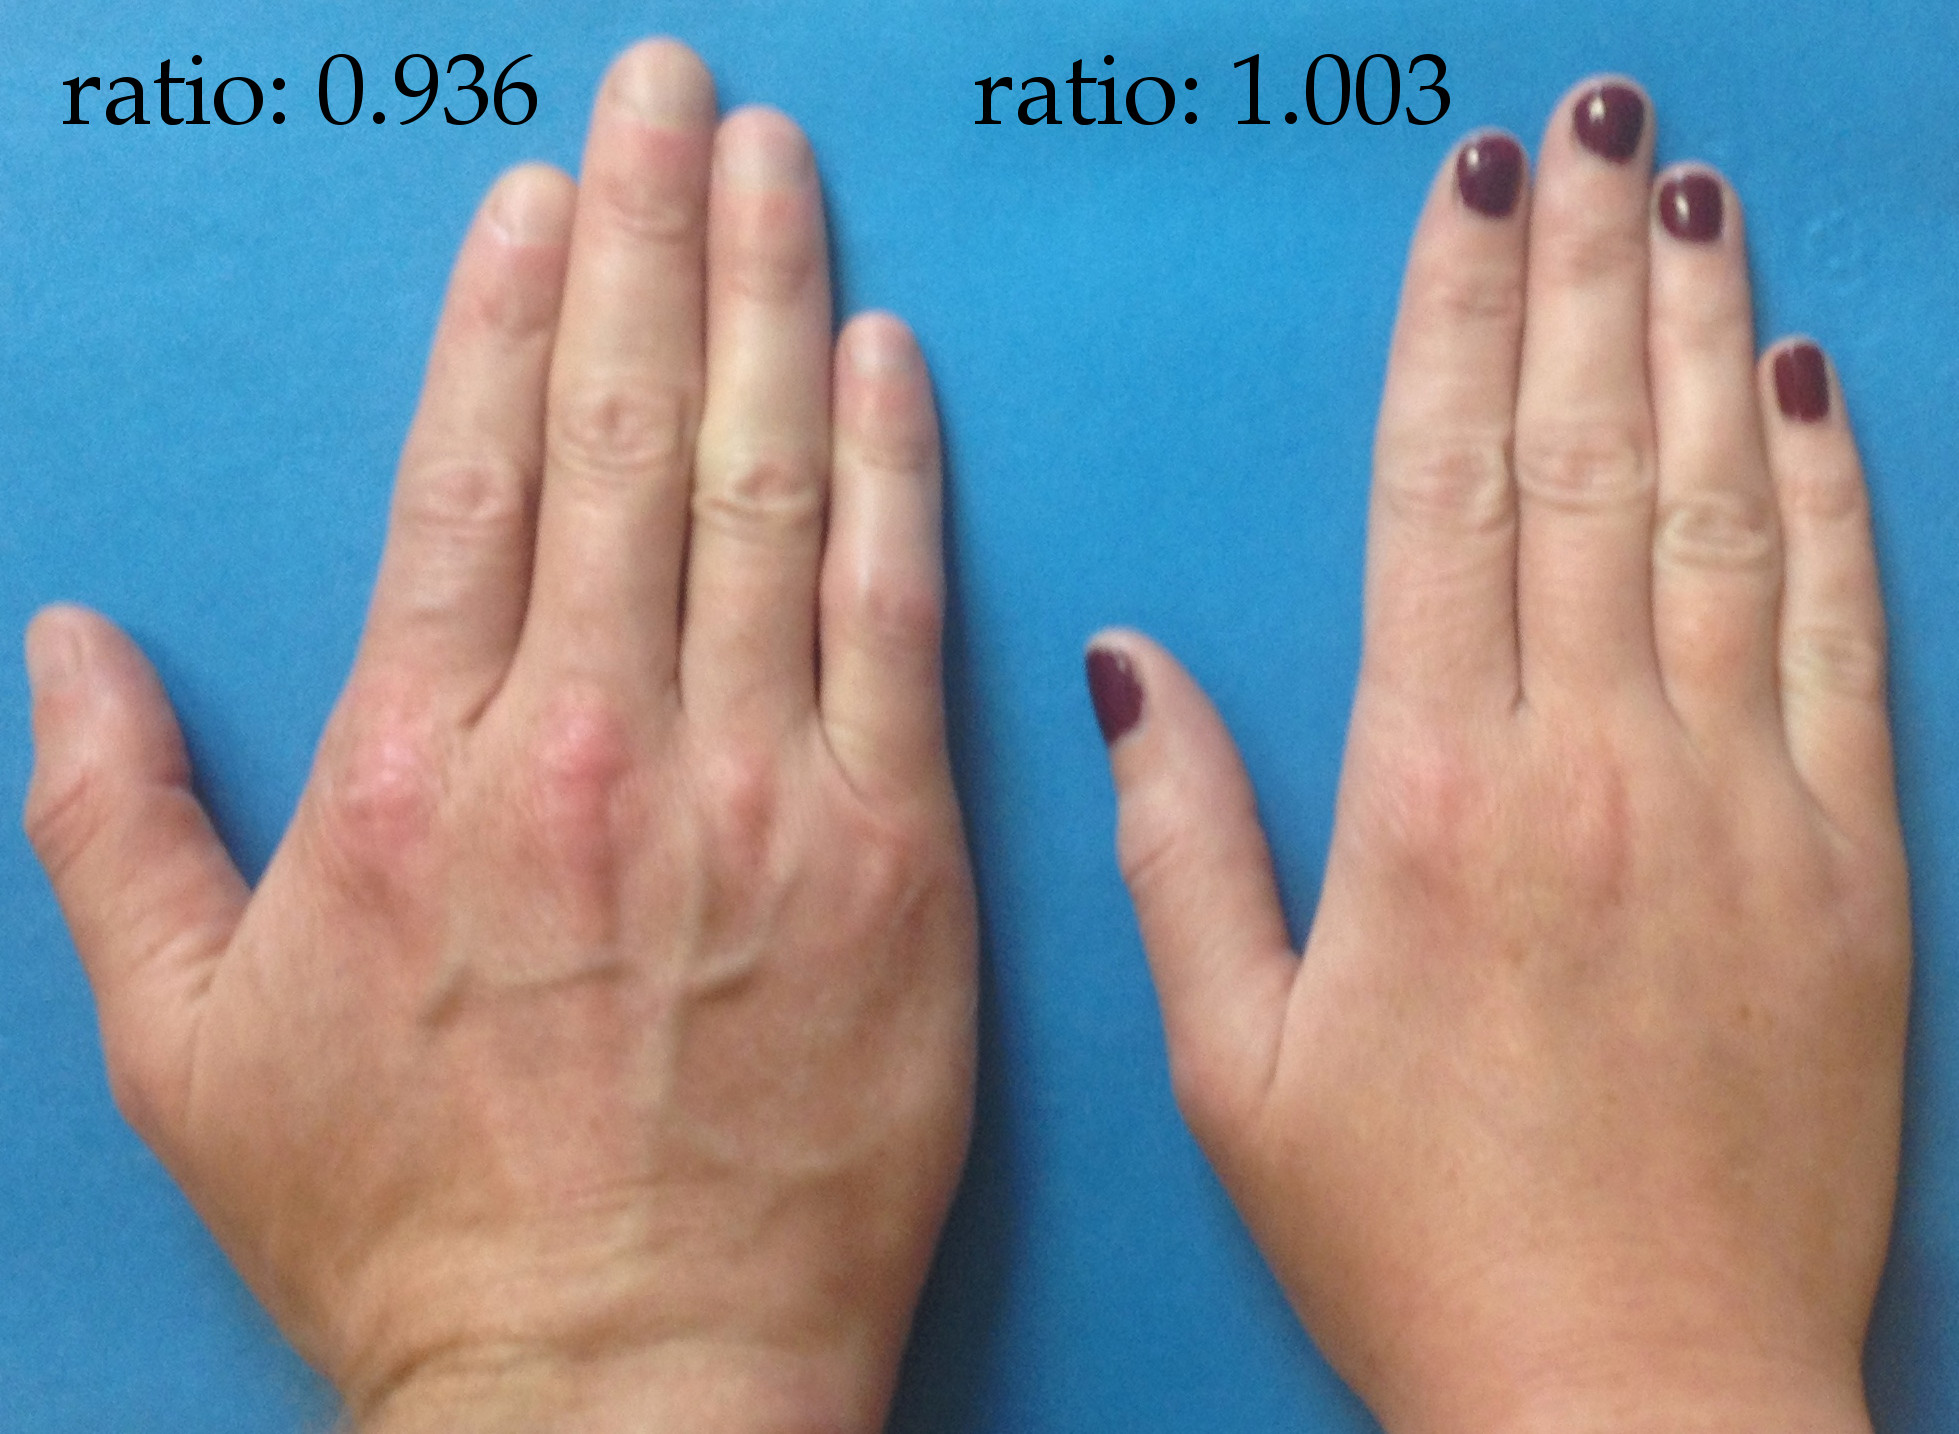
\includegraphics[width=1.12\textwidth]{realhands2.jpg}
\end{center}
\end{frame}



\begin{frame}{Phonological Specialization: \\ \small{GOOSE-NEW split in New Zealand English (Seyfarth and Sneller 2014)}}

\begin{center}
\includegraphics[width=.84\textwidth,height=.85\textheight]{../../../allophones/ByTokenOldPreceding.pdf}
\end{center}
\end{frame}


\begin{frame}{Spontaneous Phonologization: \\ \small{PRICE-raising in Philadelphia English (Fruehwald 2013)\\(308 speakers)}}

	
%\begin{center}
\includegraphics[trim=2cm 2cm 2cm 2cm, clip=false, width=.91\textwidth]{ayraisingphila.pdf}
%\end{center}

\end{frame}





\end{document}